In a nutshell, StreamFS is an analytical framework for organizing, storing, and processing streaming sensor data.
The main components of the architecture consist of a pub-sub substrate, stream operator management, and a historical
metadata manager.  The pub-sub substrate and operator manager are combined to provide a visual dataflow application
that allows a user to construct analytical processes on incoming and historical sensor data.  

Metadata management in StreamFS consists of a naming axis, a storage axis, a historical snapshot component and a query optimizer.
These pieces intersect to provide stream data context for physical sensor deployments as the physical configuration evolves over time --
a fundamental property physical sensor deployments.

\section{Open questions}
\begin{enumerate}
\item Are we really treating the metadata as a timeseries itself?  (i.e. Can we ask the same questions of the metadata that we do of typical timeseries
data?)
\item How do we perform query optimization for timeseries queries that must account for changes in the metadata over time?
\end{enumerate}

\section{Motivation, Problems, and Metrics}
In each part of the thesis work we need a good motivation for the problem, a formal articulation of the problem that 
is being addressed, and how to demonstrate that the method for addressing the problem has been successful.

\subsection{Setup and assumptions}
For this work we assume that the data is streaming is available for streaming into the system.  This assume the conversion from
a data source native format to an HTTP-POST translator has been written and is being used to push the data into StreamFS or
that the conversion has been done for pushing the data into the systems mentioned in the related-work section as alternatives.


\subsection{Problem 1:  Online analytical data processing}
Related work areas: Stream data processing, streaming queries, soft real-time

Related projects:  
\begin{itemize}
\item Dataflow programming, expression
	\begin{itemize}
	\item Ptolemy, Click
	\end{itemize}
\item Stream query scalability
	\begin{itemize}
	\item On-line Sensing Task Optimization for Shared Sensors (Arsalan Tavakoli)
	\item Scalable Delivery of Stream Query Result (Yongluan Zhou)
	\item Sensys disco (Prabal Dutta)
	\item XSense (Jorge and Prabal -- never published)
	\item SEDA (Matt Welsh)
	\item River (remzy or remzi?)
	\item Brewer's work on threading system. (Events vs Threads, etc etc)
	\item Armando (distallation - ``transcend'')
	\end{itemize}
\item General stream query processing -- in relation to dynamic queries
	\begin{itemize}
	\item Streaming Queries over Streaming Data (Sirish Chandrasekaran, Michael J. Franklin)
	\end{itemize}
\item Horizontally scaling the namespace and processing across machines
	\begin{itemize}
	\item How do you run queries across namespaces?
	\item is there a way to join namespaces into one larger namespace?
	\item can you move computation around?  (closer to where the data is)
	\end{itemize}
\end{itemize}

\subsubsection{Metrics}
{\bf Scalability}:  How many simultaneous flows can we support?  Processing?  Delivery?

We want to be able to scale as the number of incoming flows increases, the number of processing element (threads) increases, and the number of forwarding
targets increases.  What mechanisms are in place to scale automatically?  How much sharing can we do between dynamic queries? {\bf Dynamic queries} are
useful, but they lead to problems with scalability.  What mechanisms exist to deal with scaling \emph{dynamic queries}.

{\bf Delivery} Scaling the delivery of reports to targets:
\begin{enumerate}
\item Get the report times to overlap
	\begin{itemize}
	\item Scheduling algorithm for maximum overlap.
	\item Constraints include strict periodicity +/- epsilon
	\end{itemize}
\item Consolidate readings into JSON
\item Compress the delivery and send it to target
\item Offer local buffering
	\begin{itemize}
	\item Design fetch protocol where buffer fetch and kept if necessary.  Shared buffer only accessible by specified target (same hostname/ip)
		or client explicitly specified as a fetcher.
	\item buffer size could be specified in request
	\end{itemize}
\end{enumerate}

* Take readings and do the interpolation and compare with the data quality of the result oif you don't do that. -- go into that with the smap 
data that's available in the building

* Solve the metadata problem -- it's really important
	- caveat -- doing it with the tree/hierarchy thing might make it pretty hard
	- mobility under TCP problem (handoff)
	- INS, Internet indirection
	
{\bf Corner cases include}:
\begin{itemize}
\item delivery-time difference drift (the difference between the delivery time of the next 
	delivery for a pair of schedules changes over time -- often it cycles).  We need a mechanism for dealing
	with this.  Example:  [period=2, start\_time=0], [period=3, start\_time=1]
\end{itemize}

{\bf Expressivity}:  How does this compare against the traditional way of setting up the analytical pipeline?  (lines of code?)
What are the types of analytical tasks that we want to construct and how does it compare to the alternative?


\subsection{Problem 2: Slicing, dicing, and molding data}
Referred to by David Culler as producing distillates of the data.  In particular, the processing model is in the context of moving
data and stationary operators.  For example, you write the interpolator and aggregator to run on moving/buffered windows of data.

{\bf TODO}: generalize the backend fetch.

Related work areas:  OLAP (online analytical processing), OLTP	

\subsubsection{Metrics}
{\bf Query speed}: In referring to query speed, we compare the query speed of running the typical OLAP queries on the historical
data.

\subsection{Problem 3: Metadata management}
No prior work in the management of timeseries metadata.

Using the sfs data model, we need to maintain two main data structures:
\begin{enumerate}
\item metadata map
\item node properties
\end{enumerate}

As a third component, we maintain timeseries data produced by the stream resources in the system.  Queries along the data-time dimension
must be merged across the mmap time-dimension and the node-properties time-dimension.\\

{\bf Solution outline}: The general approach here is to timestamp each node, identified by a path in the mmap.  There are up to two timestamps
for each node.  1)  the timestamp at the point of creation and 2) the timestamp at the point of deletion.\\

{\bf Challenges}:
\begin{itemize}
\item Query that goes back to a particular point in time.
\item Dynamic query that goes back to a particular point in time and walks forward to the current time (any kind of aggregation
query that uses all the items in a particular context over time).  This is especially challenging because of symbolic links.\\
\end{itemize}


{\bf Queries to consider are}:
\begin{itemize}

\item {\bf Was the database ever in a particular state?} (i.e.Did this room ever contain a laptop belonging to jorge?)
\item timeseries query from now to some point in time where there were no changes in properties, but there was in naming, and data
\item timeseries query from now to some point in time where there were changes in properties and data, but not naming
\item timeseries query from now to some point in time where there were changes in properties, data, and naming
\item query that sets now to some point in time in the past
\item operators that are provided with the different types of queries:
	\begin{itemize}
	\item filter by property type and aggregate (sum values)
	\item filter by property type, interpolate, aggregate\\
	\end{itemize}
\end{itemize}

Baseline performance should be compared with doing a standard query on timeseries data.  What's the overhead for performing
each of these types of queries.  {\bf In-time queries} run immediately and should have queries latency comparable to a standard
timeseries query.  {\bf Dynamic queries} run forever (until they are uninstalled) and should have query latencies reasonable consistent
and close to the time that data was received from each query.  Dynamic queries handle changes in naming, properties, and data.
{\bf Continuous queries} are the simpler version of dynamic queries.  No changes to naming and properties has occurred.  There are 
only changes to the data -- it is continuously streaming in from a particular data source.

According to~\cite{temporal_dbs}, there are four type of databases that deal with time.
\begin{enumerate}
\item snapshot
\item rollback
\item historical
\item temporal\\
\end{enumerate}
Snapshot databases are databases where each operation performed on the db overwrite the previous state before the operation
was committed; yielding the latest snapshot of the database.  Rollback databases are collections of snapshots.  To run a query
at a particular point in the past is to rollback the database and run the query on the active snapshot at that point in time.
Once the state is rolled forward, past snapshot states cannot be altered.  The main drawback here is that {\bf updates to past states
cannot be corrected once the snapshot is produced.}  Historical databases are concerned only with relations, or facts, with respect
to when they were true in the real world.  It is not concerned with the time when the fact was stored in the database itself.  For example,
Jorge has lived in Berkeley since August 21, 2005 and will move out on September 30, 2011.  This is the time for which this fact is true,
even if this fact was stored today, August 30, 2011.  When it was stored is irrelevant.  Temporal databases combine rollback and historical,
combining transaction time and valid time, supporting retro/proactive queries.  User-defined time should also be handled, doubling the
kinds of databases.


\begin{figure*}[tb!]
\begin{center}
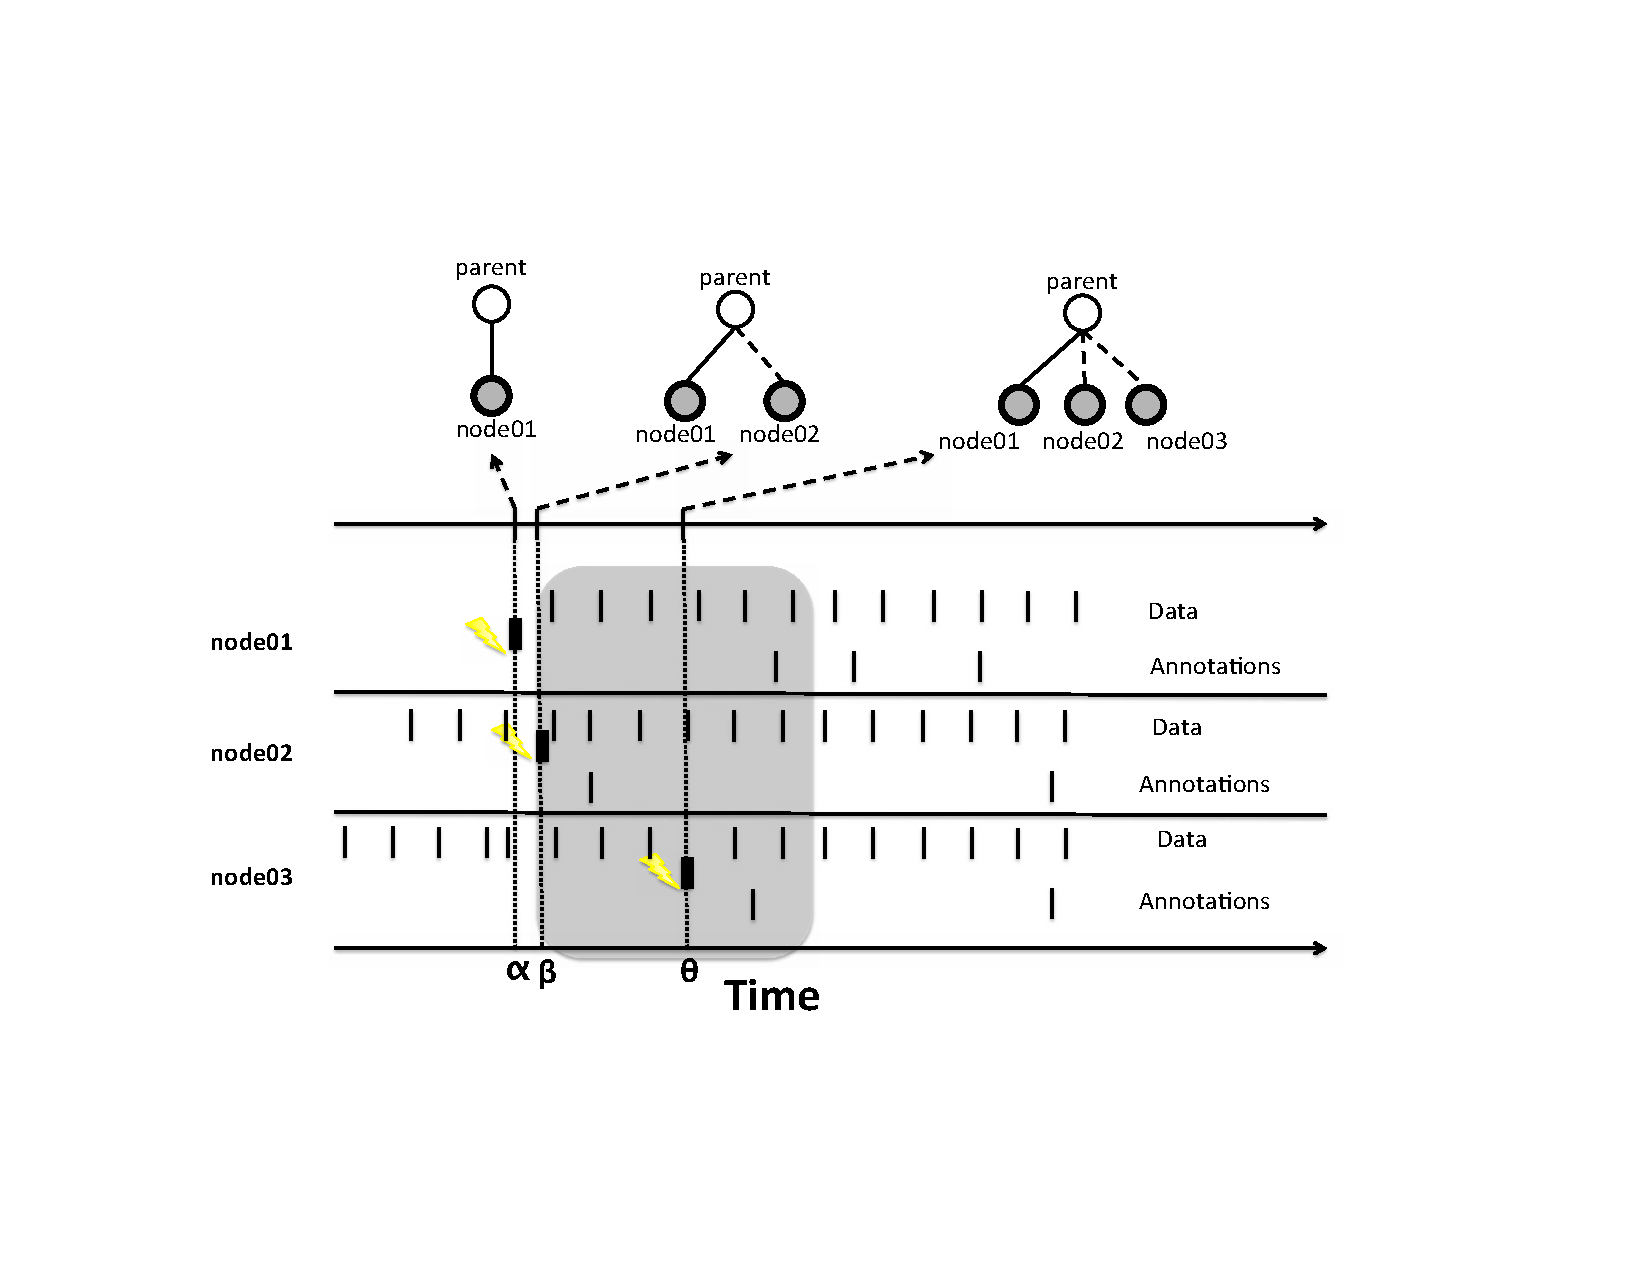
\includegraphics[width=0.75\textwidth,height=2.2in]{plots/mtsq}
%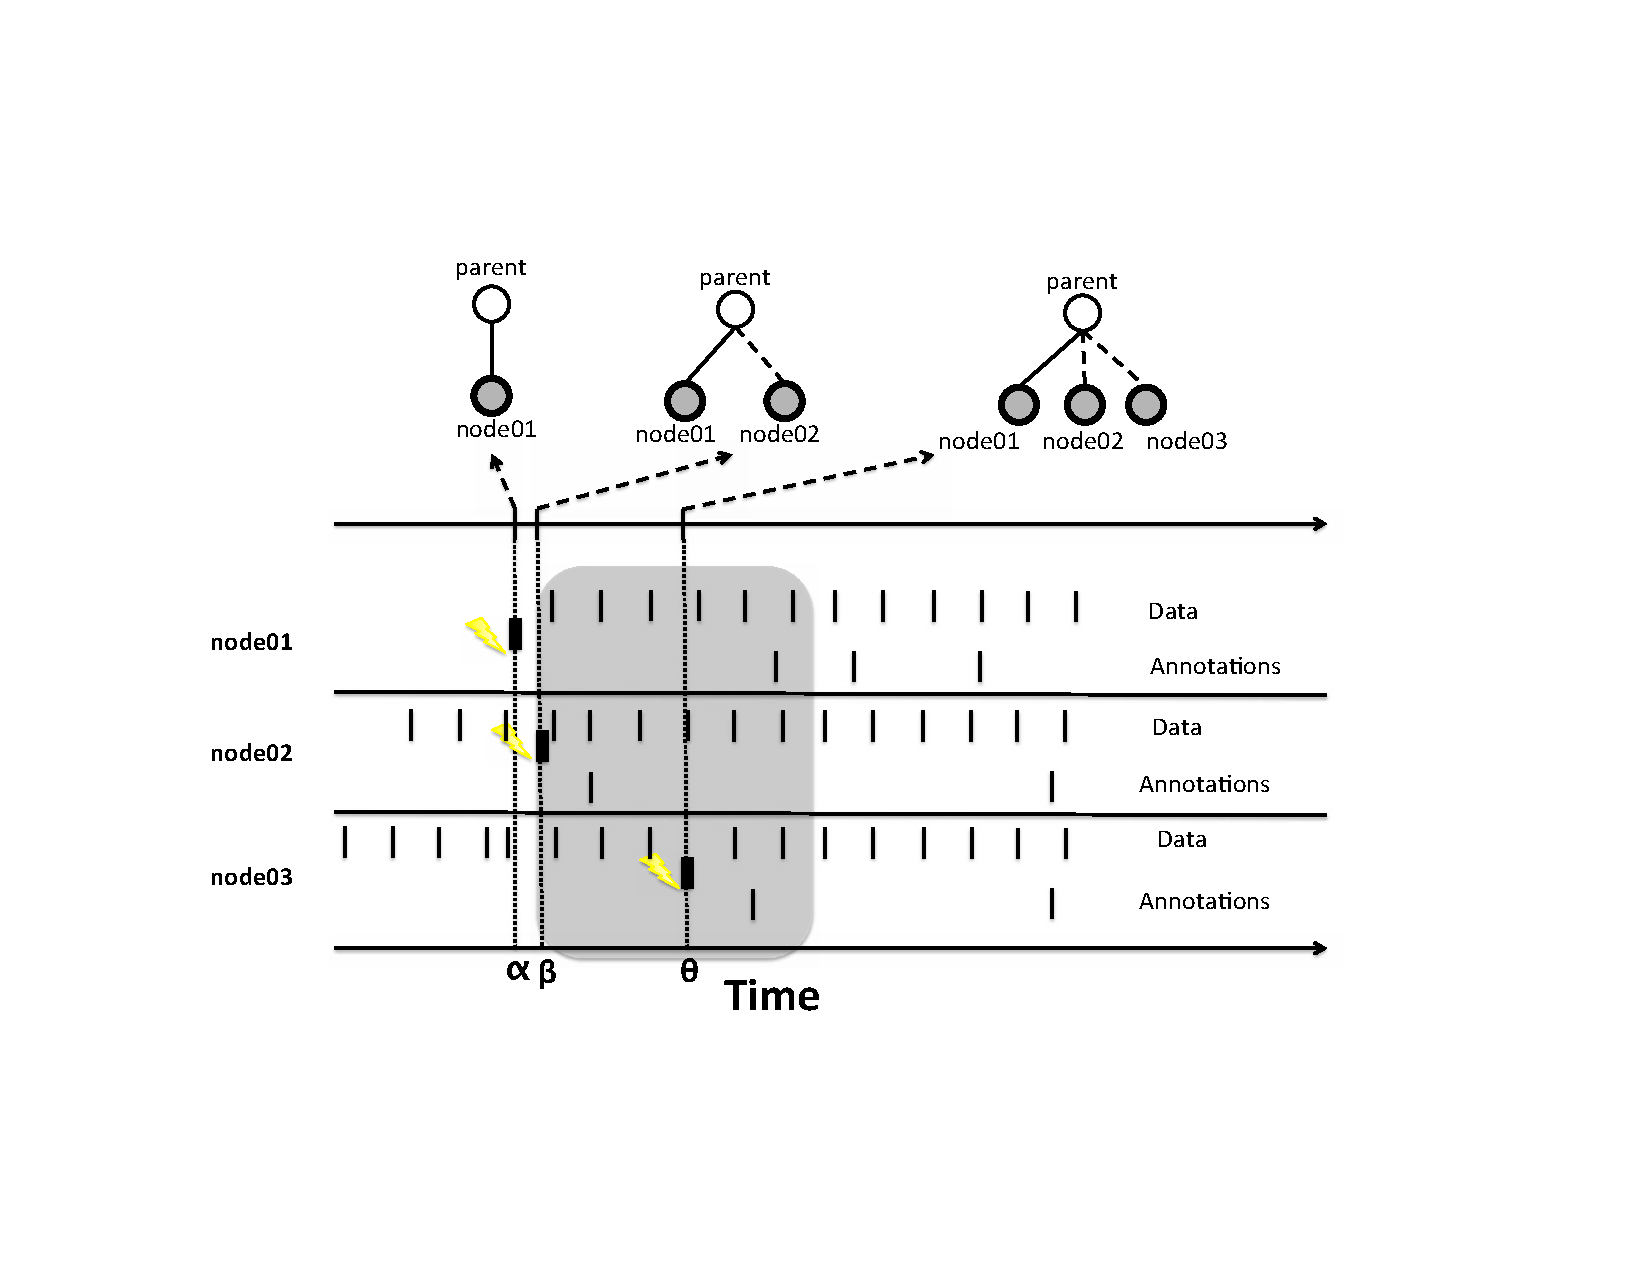
\includegraphics[width=0.65\textwidth]{plots/mtsq}
\caption{}
\vspace*{-5mm}
\label{fig:timestitch}
\end{center}
\end{figure*}


\subsection{Problem 4: Global object lookup}
Object identifer with version numbers as fundamental aspect of the namespace.

%related work
%
% http://citeseerx.ist.psu.edu/viewdoc/summary?doi=10.1.1.105.3673 -- Chord lookup
% http://citeseerx.ist.psu.edu/viewdoc/summary?doi=10.1.1.41.2924
% http://citeseerx.ist.psu.edu/viewdoc/summary?doi=10.1.1.17.339


























